外径50 \si{[\mm]}、内径10 \si{[\mm]}の円筒内に満たされている水が全て凍結するまでの時間を
後退差分法のVTS法で求めるプログラムをソースコード\ref{s1}に示す。
各時間ステップを出力したものを実行結果として、図\ref{im1}~\ref{im4}に示す。\\

\begin{lstlisting}[caption=円筒状物体が凍結するまでの時間を後退差分法のVTS法で求めるプログラム,label=s1]
#include <stdio.h>
#include <math.h>

#define N 100
#define lambda_s 2.22
#define cp_s 2067
#define rho_s 917
#define alpha_s lambda_s / (rho_s * cp_s)
#define L 334880
#define Ta -5
#define Tm 0
#define A 0.005
#define B 0.025
#define eps 1e-5

double dt[N], old_dt[N];
double t_s[N][N] = {Tm};

const double dr = (B - A) / N; // drの算出

void thomas_init(int n, double a[], double b[], double c[], double d[]){
  double r_s = (alpha_s * dt[n]) / (dr * dr);

  for(int i=0;i<n;i++){
    a[i] = -r_s * (1 - 1 / (2 * (A / dr + i + 1)));
    b[i] = 1 + 2 * r_s;
    c[i] = -r_s * (1 + 1 / (2 * (A / dr + i + 1)));
    d[i] = t_s[i+1][n];
  }
  d[0] = t_s[1][n] + r_s * (1 - 1 / (2 * (A / dr + 1))) * Ta;
  d[n-1] = 0;
}

void thomas(int n, double a[], double b[], double c[], double d[]){
  for(int i=1;i<n;i++){
    double e = a[i] / b[i-1];
    b[i] = b[i] - e * c[i-1];
    d[i] = d[i] - e * d[i-1];
  }
  d[n-1] = d[n-1] / b[n-1];
  for(int i=n-2;i>=0;i--){
    d[i] = (d[i] - c[i] * d[i+1]) / b[i];
  }

  for(int i=1;i<=n;i++){
    t_s[i][n+1] = d[i-1];
  }
}

int is_convergence(double old_val, double new_val) {
  // 収束判定
  double e_temp = fabs((new_val - old_val) / old_val);
  if(e_temp > eps){
    return 1;
  } else {
    return 0;
  }
}

int main(){
  double t_sum = 0;
  for(int i=0;i<N;i++) {
    dt[i] = 0;
    old_dt[i] = 0;
  }

  // dt_0
  t_s[0][1] = Ta;
  dt[0] = ((rho_s * L) / lambda_s) * ((dr * dr) / (Tm - Ta));
  printf("Δt_0  = %7.3lf[s]\n", dt[0]);
  t_sum += dt[0];

  // dt_1
  dt[1] = dt[0];
  do {
    old_dt[1] = dt[1];

    double r_s = (alpha_s * dt[1]) / (dr * dr);
    double q = 1 / (2 * (A / dr + 1)); // t_s1計算の簡略化変数
    t_s[1][2] = 1 / (1 + 2 * r_s) * ((1 + r_s * (1 + q)) * Tm + r_s * Ta * (1 - q));
    dt[1] = ((rho_s * L) / lambda_s) * ((dr * dr) / (Tm - t_s[1][2]));
  } while(is_convergence(old_dt[1], dt[1]));
  printf("Δt_1  = %7.3lf[s]\n", dt[1]);
  t_sum += dt[1];

  // dt_2 ->
  for(int i=2;i<N;i++){
    dt[i] = dt[i-1];
    double a[i], b[i], c[i], d[i];

    do {
      old_dt[i] = dt[i];

      thomas_init(i, a, b, c, d);
      thomas(i, a, b, c, d);
      dt[i] = ((rho_s * L) / lambda_s) * ((dr * dr) / (Tm - t_s[i][i+1]));
    } while(is_convergence(old_dt[i], dt[i]));

    printf("Δt_%-2d = %7.3lf[s]\n", i, dt[i]);
    t_sum += dt[i];
  }

  printf("\nt = %7.3lf[s]\n", t_sum);
  return 0;
}
\end{lstlisting}

\begin{figure}[H]
  \begin{center}
    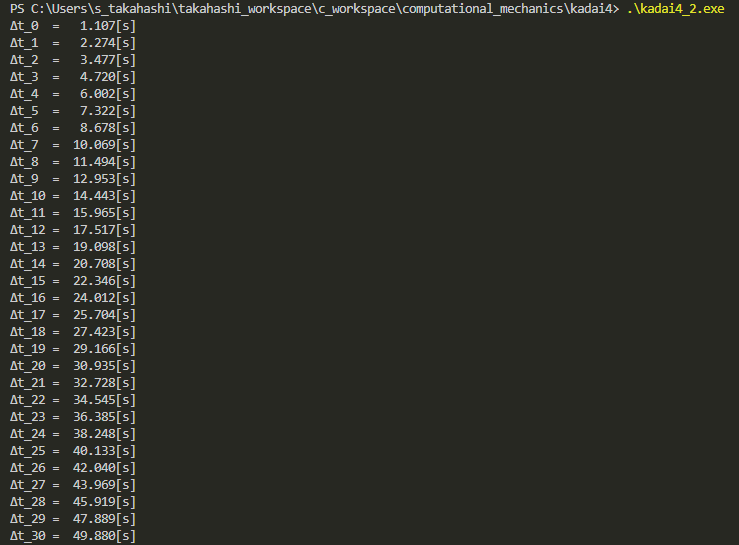
\includegraphics[width=.8\linewidth]{img/k4_1.png}
    \caption{実行結果1}
    \label{im1}
  \end{center}
\end{figure}
\begin{figure}[H]
  \begin{center}
    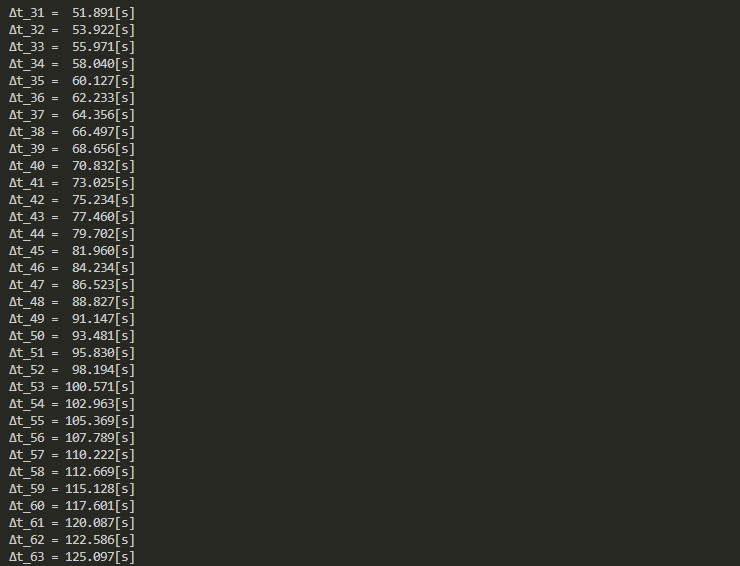
\includegraphics[width=.8\linewidth]{img/k4_2.png}
    \caption{実行結果2}
    \label{im2}
  \end{center}
\end{figure}
\begin{figure}[H]
  \begin{center}
    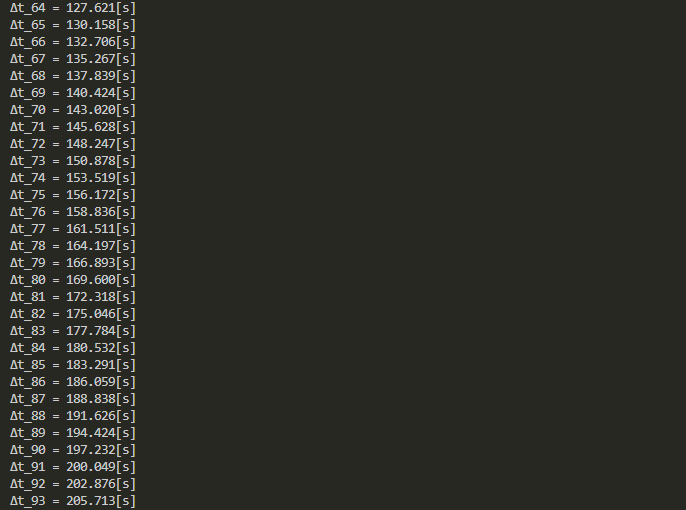
\includegraphics[width=.8\linewidth]{img/k4_3.png}
    \caption{実行結果3}
    \label{im3}
  \end{center}
\end{figure}
\begin{figure}[H]
  \begin{center}
    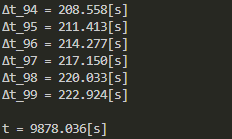
\includegraphics[width=.8\linewidth]{img/k4_4.png}
    \caption{実行結果4}
    \label{im4}
  \end{center}
\end{figure}